\section{Star Partition and Mining}
\label{sec:spm_solution}
In order to develop a method that achieves good parallelism under any pattern parameters, 
we propose the \emph{Star Partition and Mining} (SPM) method. In SPM,
we first design a novel object-based partition method named \emph{star partition}. 
Then, we design an \emph{Apriori}-like 
method to mine GCMP patterns out of each partition.
The overview of the SPM method is presented in Algorithm~\ref{algo:spm_overview}.
As shown, the SPM method takes three phases. 
In the map phase, objects from the same cluster forms object-object pairs. 
The object-object pairs are then paired up with the timestamp of 
the snapshot to form a 3-uple(lines~\ref{code:spm-map-start}-\ref{code:spm-map-end}). 
In the partition phase, 3-uples with the same leading object form a \emph{star} which will be explained shortly 
(lines~\ref{code:spm-shuffle-start}-\ref{code:spm-shuffle-end}).
Lastly in the reduce phase, patterns are mined from each star structure (lines~\ref{code:spm-reduce-start}-\ref{code:spm-reduce-end}).

\begin{algorithm}
\caption{Star Partition and Mining}
\label{algo:spm_overview}
\begin{algorithmic}[1]
\Require list of $\langle t, S_t \rangle$ pairs
\State {---Map phase---}
\label{code:spm-map-start}
\ForAll{$C \in S_t$}
	\ForAll {$(o_1 ,o_2) \in C \times C$}
		\If{$o_1 < o_2$}  \label{code:spm-edge-direct}
			\State emit a $\langle o_1, o_2, \{t\}\rangle$ triplet
		\EndIf
	\EndFor
\EndFor
\label{code:spm-map-end}

\State {---Partition and Shuffle phase---}
\label{code:spm-shuffle-start}
\ForAll{$\langle o_1, o_2, \{t\}\rangle$ triplets} 
	\State group-by $o_1$, emit $\langle o_1, Sr_{o_1} \rangle$ 
	%\State group-by $o_2$, emit $\langle o_2, Sr_{o_2} \rangle$
\EndFor
\label{code:spm-shuffle-end}

\State {---Reduce phase---}
\label{code:spm-reduce-start}
\ForAll{$\langle o, Sr_{o} \rangle$}
\State Apriori($Sr_o$)
\EndFor
\label{code:spm-reduce-end}

\end{algorithmic}
\end{algorithm}

\subsubsection{Star Partition}
The intuition of star partition is that, if two objects are part of
the same pattern, then at some snapshots, they must belong to the same 
cluster. Therefore, we may link objects that belong to the same cluster
at some snapshots to form a \emph{connection graph}. Objects that are
not connected surely do not belong to a pattern. We may further
partition the connection graph so that mining proper patterns can be
done in parallel. We define the \emph{connection graph} and \emph{star}
as follows:
\begin{definition}[Connection Graph and Star]
A connection graph is an undirected graph $G=(V:E)$, where 
each $v \in V$ represents an object. An edge $e(s,t)= ET \in E$ 
contains all the timestamps at which $s,t$ are in the same cluster,
i.e., $\forall t \in ET, C_t(s) = C_t(t)$. 
A star of a vertex $s$, denoted as $Sr_s$, is the set of incidental edges on $s$ whose
another ending vertex is greater than $s$. I.e, $\forall e(s,t) \in Sr_s$, $s < t$. We name $s$
as the \emph{central vertex} of $Sr_s$.
\end{definition}

It is notable that we require vertices in a star to be greater than its central vertex. This 
effectively avoids replicating edges. \emph{Connection graph} and \emph{star} examples are 
shown in Figure~\ref{fig:star_partition} (a) and (b). In (a), a connection graph is formed
based on the example in Figure~\ref{fig:related_work}.
In (b), 5 stars are presented. It is easy to see that, by requiring the center vertex to be
the smallest vertex in a star, there are no edges been replicated. In implementation,
as stated in Algorithm~\ref{algo:spm_overview} line~\ref{code:spm-edge-direct}, the
comparison between vertices/objects are based on the vertex/object ID.

\begin{figure}[h]
\centering
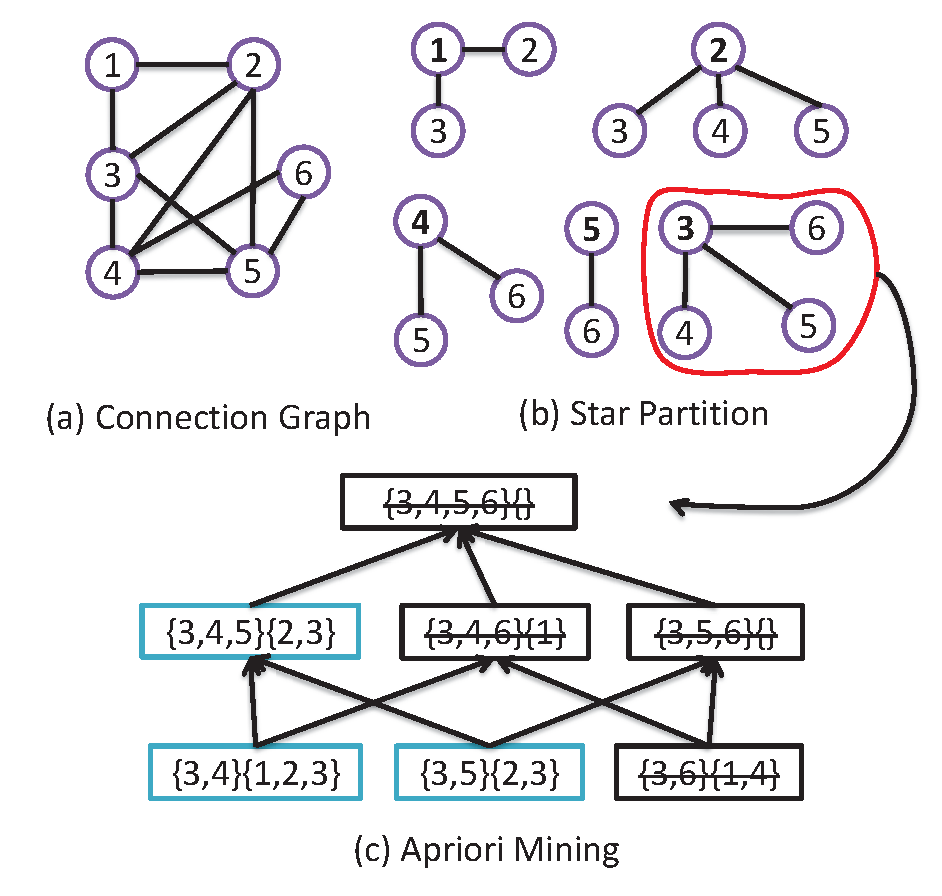
\includegraphics[width=0.4\textwidth]{spm.eps}
\caption{Star partition and mining of trajectories in Figure~\ref{fig:related_work}}
\label{fig:star_partition}
\end{figure}

%After computing the star, each partition is applied with a reduce task. 
%Indeed, a star $Sr_s$ can be viewed as a subset of original trajectories. 
%This is done by treating each vertex in $Sr_s$ as an object. 
%The time sequence of $s$ is the union of all edges in $Sr_s$. 
%And the time sequence of $v \neq s$ is the edge $(s,v)$. Therefore, we
%are able to mine stars from the similar trajectory concepts.
Although star partition is performed based on the object connections, each star
can be effectively viewed as a subset of trajectories. To see this, each vertex
in a star can be viewed as an object. The timestamps of center vertex $s$ is the
union of all the edges in $Sr_s$. The timestamps of vertex $v \neq s$ is the 
edge $e(s,v)$. Therefore, we are able to define and mine GCMP on the stars. 
Before describing the mining strategy, we first state in the following theorem that 
the star-partition is complete and sound:
\begin{theorem}[Soundness and Completeness of Star Partition]
Star partition is sound and complete.
\end{theorem}

\begin{proof}
For the soundness,
if $P$ is a valid pattern in $Sr_s$, then at every time $t$, $\forall o_1, o_2 \in P.O$, $C_t(o_1) = C_t(o_2)$.
By definition, $P$ is valid in the original trajectories.
For the completeness,
if $P$ is a valid pattern in original trajectories, let $s$ be the object with smallest ID in $P.O$. 
Then by the definition of pattern, $\forall t \in P.T$, $\forall o \in P.O$, $C_t(s) = C_t(o)$.
It follows that all object $o \in P.O$ are in $Sr_s$. Furthermore, every timestamp in $P.T$ is included
in $Sr_s$. Therefore, $P$ is a valid pattern in $Sr_s$.
\end{proof}

Based on the above theorem, we can mine GCMP from each partition independently.
It is notable that, in star partition, original data is replicated for $O(\mathbb{O})$ times
as each object may be sent to $O(\mathbb{O})$ partitions. Since this complexity is free
from pattern parameters, the star partition is more scalable than the temporal replication.
In later sections, we will describe several engineering level optimization to further reduce the amount of replicated data.

\subsubsection{Apriori Mining}
In the mining phase, we need to find the patterns within each star. 
To systematically discover the patterns, we design the \emph{Apriori Mining} method which
is similar to the technique in frequent item mining literature. During the algorithm, we call a candidate pattern $R$-pattern if the size of its object set is $R$. 
Our algorithm runs in iterations. During each iteration $R$, we try to generate all $(R+1)$-patterns. In iteration $1$, the $2$-pattern is the edges in $Sr_s$. In particular,
for each $e(s,v)=ET$, pattern $p=(\{s,v\}, ET)$ is formed. During each iteration, 
we generate $(R+1)$-patterns by joining $R$-patterns with $2$-patterns. Specifically,
the join between $p_1=(O_1, T_1)$ and $p_2=(O_2, T_2)$ would generate a new pattern $p_3=(O_1 \cup O_2, T_1 \cap T_2)$. Notice that in $Sr_s$, each $R$-pattern consists of the object $s$, thus the join will grow a $R$-pattern at most to a $(R+1)$-pattern.
Our mining algorithm stops where no further patterns are generated. The algorithm is illustrated as in Algorithm~\ref{algo:apriori_mining}.

\begin{algorithm}
\caption{Apriori Mining}
\label{algo:apriori_mining}
\begin{algorithmic}[1]
\Require{$Sr_s$}
\State { Lv $\gets \{\}$}
\State { Ground $\gets \{\}$}
\ForAll{$e(s,t) = T \in Sr_s$}
\State Ground.add($\langle \{s,t\}, T \rangle$);
\State Lv $\gets$ Ground;
\EndFor
\While{true}
	\If{Lv is not empty} 
		\State{LvCand $\gets \{\}$ }
		\ForAll{$cand_v \in Lv$}
			\ForAll{$cand \in $Ground}
				\State $p \gets cand_v$ join $cand$
				\If{$p.T$ is partly valid} 
					\State LvCand.add($p$)
				\EndIf
			\EndFor
		\EndFor
		\State {Lv $\gets$ LvCand}
	\Else
		\State{break}
	\EndIf
\EndWhile
\end{algorithmic}
\end{algorithm}

An illustration of Algorithm~\ref{algo:apriori_mining} is shown in Figure~\ref{fig:star_partition} (c).
As shown, the star $Sr_3=\{3,4,5,6\}$ initially generate three $2$-candidates. At every iteration, 
higher level candidates are generated by joining lower level candidates. When no more candidates 
can be generated, the algorithm stops by outputting the valid patterns.

It is notable that Algorithm~\ref{algo:apriori_mining} takes exponential complexity to mine GCMP. There
are two major factors dragging down the performance. First, the size of $Sr_s$ affects
the initial size of $2$-patterns. Second, the candidates generated in each level affects the join performance. In later
sections, we exploit the property of GCMP to reduce the two factors.
